\documentclass[12pt]{report}

% These twolines are needed by the epydoc generated files
\usepackage{alltt}
\usepackage{makeidx, multirow, longtable, tocbibind, amssymb}

\usepackage{url}
\usepackage{geometry}
\geometry{letterpaper}
\usepackage[parfill]{parskip}
\usepackage{graphicx}
\usepackage{fancyhdr}

\newlength{\BCL} % base class length, for base trees.

\pagestyle{fancy}
\headheight 15pt

\title{\bf NetWorkSpaces for Matlab \\ User Guide \\ \rm \it Version 1.3}
\author{REvolution Computing, Inc. \\ http://www.lindaspaces.com}

\begin{document}
\maketitle
\tableofcontents

\chapter{Introduction}
NetWorkSpaces (NWS) provides a framework to coordinate programs written
in scripting languages; NWS currently supports the languages Python,
MATLAB, and R.  This User Guide is for the MATLAB system, and it
assumes that the reader is familiar with MATLAB.

\section{Data Sharing}
A MATLAB program uses variables to communicate data from one part of the
program to another.  For example, \texttt{x = 123} assigns the value 123
to the variable named \texttt{x}.  Later portions of the program can
reference \texttt{x} to use the value 123.  This mechanism is generally
known as \textit{binding}.  In this case, the binding associates the
value 123 with the name \texttt{x}.  The collection of name-value
bindings in use by a program is often referred to as its
\textit{workspace}.

Two or more MATLAB programs use NWS to communicate data by means of
name-value bindings stored in a network-based workspace (a netWorkSpace,
which in MATLAB is an instance of a netWorkSpace object).  One program
creates a binding, while another program reads the value the binding
associated with the name. This is clearly quite similar to a traditional
workspace; however, a netWorkSpace differs from a traditional workspace
in two important ways.

First, in a setting in which two or more MATLAB programs are
interacting, it would not be unusual for one to attempt to ``read'' the
value of a name before that name has been bound to a value.  Rather than
receiving an ``unbound variable'' error, the reading program (by default)
simply waits (or ``blocks'') until the binding occurs. Second, a common
usage paradigm involves processing a sequence of values for a given
name. One MATLAB program carries out a computation based on the first
value, while another might carry out a computation on the second, and so
on. To facilitate this paradigm, more than one value may be bound to a
name in a workspace and values may be ``removed'' (fetch) as opposed to
read (find). By default, values bound to a name are consumed in
first-in-first-out (FIFO) order, but other modes are supported:
last-in-first-out (LIFO), multiset (no ordering implied) and single
(only the last value bound is retained). Since all its values could be
removed, a name can, in fact, have no values associated with it.

A netWorkSpace provides five basic operations:
\textbf{store}, \textbf{fetch}, \textbf{fetchTry}, \textbf{find}, and
\textbf{findTry}:
\begin{description}
\item[store] introduces a new binding for a specific name in a given workspace.
\item[fetch] fetches (removes) a value associated with a name, blocking
if necessary until a value is available.
\item[fetchTry] fetches (removes) a value associated with a name without
blocking.
\item[find] reads a value without removing it, blocking if necessary.
\item[findTry] reads a value without removing it and without blocking.
\end{description}

Note that \textbf{fetchTry} and \textbf{findTry} return \texttt{0} or
a user-supplied default if no value is available.

There are several additional netWorkSpace operations:
\begin{description}
\item[currentWs] returns the name of the specified workspace.
\item[declare] declares a variable name with a specific mode.
\item[deleteVar] deletes a name from a workspace.
\item[listVars] provides a list of variables (bindings) in a workspace.
\end{description}

In addition to a netWorkSpace, a MATLAB client of NWS also uses an
nwsServer object. This object is created automatically when a new
netWorkSpace object is created, so you don't need to interact directly
with it. However, the \texttt{server} method provides access to the
nwsServer object:

\begin{verbatim}
>> ws = netWorkSpace('foo')
>> server(ws)
\end{verbatim}

A nwsServer object supports the following actions:

\begin{description}
\item[openWs] connects to a workspace or creates one if the specified
workspace does not exist. 
\item[useWs] uses a netWorkSpace without claiming ownership.
\item[deleteWs] explicitly deletes a workspace.
\item[listWss] provides a list of workspaces in the server.  
\item[close] closes the connection to a workspace. Depending on the
ownership, closing a connection to a workspace can result in removing
the workspace. 
\end{description}

\section{Parallel Computing}
The operations above enable coordination of different programs using
NWS. There is also a mechanism, built on top of NWS, called Sleigh
(inspired by R's SNOW package) to enable parallel function evaluation.
Sleigh is especially useful for running {\it embarrassingly parallel}
programs on multiple networked computers. Once a sleigh is created by
specifying the nodes that are participating in computations, you can
use:

\begin{description}
\item[eachElem] is used to execute a specified function multiple times
in parallel with a varying set of arguments.
\item[eachWorker] is used to execute a function exactly once on every
worker in the sleigh with a fixed set of arguments.
\end{description}

Various data structures (workspaces, name-value bindings, etc.) in a NWS
server can be monitored and even modified using a web interface. In
distributed programming, even among cooperating programs, the state of
shared data can be hard to understand. The web interface presents a
simple way of checking current state remotely. This tool can also be
used for learning and debugging purposes, and for monitoring ``normal''
MATLAB programs as well.


\chapter{Getting Started}
This chapter provides procedures for setting up NetWorkSpaces
and Sleigh for MATLAB.  See the INSTALL and README files in the
NetWorkSpaces distribution for more information.

\section{Prerequisites}
NetWorkSpaces runs on Linux, Max OS X, Windows, and most Unix systems.
The MATLAB NWS API has no prerequisites, other than MATLAB 7.0 or later.
However, you must be running a NetWorkSpaces server on some network
accessible machine (which includes the local machine, of course).  The
server is a Python/Twisted application, and therefore requires Python
with Twisted installed.  NetWorkSpaces uses Twisted Core and Twisted
Web, and Twisted in turns requires Zope Interfaces, which comes bundled
with the Twisted installation.

To summarize:
\begin{itemize}
\item MATLAB 7.0 or later \url{http://www.mathworks.com}
\item Python 2.2 or later \url{http://www.python.org}
\item NetWorkSpaces server \url{http://nws-py.sourceforge.net}
\item Twisted Core 2.1 or later \url{http://twistedmatrix.com}
\item Twisted Web 0.5 or later
\item Zope Interfaces (as distributed with Twisted)
\end{itemize}

Note on Windows, NetWorkSpaces has an ``all-in-one'' installer that will
install everything that you need to run the server, MATLAB~NWS~API,
Python~NWS~API, and R~NWS~API, so if you choose to use that, you don't
have to be aware of these software requirements.

\section{NetWorkSpaces Server}
\subsection{Starting the Server}
There are several ways to start a NetWorkSpaces server.
If you install NetWorkSpaces on Windows with the ``all-in-one''
installer, than the server is already running as the
``NwsService''.  You can check on it's status, start, and stop it using
the standard Windows tools.

\begin{itemize}
\item {twistd command (as daemon):}
\begin{verbatim}
% twistd -y /etc/nws.tac
\end{verbatim}

Note: nws.tac is installed in different directories, depending on
the platform and the type of installation (root versus non-root).
For root installation, nws.tac is located in \texttt{/etc} on UNIX,
and in the PYTHON24 or PYTHON25 directory on Windows. 
\item {nws script (UNIX only):} \\
The nws script is intended to be an init script, but it can be
used manually, as follows:
\begin{verbatim}
% nws start
\end{verbatim}
\item {NwsService (Windows only):} \\
If you didn't install NetWorkSpaces using the ``all-in-one'' installer, the
procedure installing and running the service is:
\begin{enumerate}
\item Open up a command prompt
\item Install NwsService by executing NwsService.py, which is located in Python's scripts directory
\begin{verbatim}
C:\python25\scripts> python NwsService.py install
\end{verbatim}
\item Start NwsService
\begin{verbatim}
C:\> sc start nwsservice
\end{verbatim}
\end{enumerate}
\end{itemize}

\subsection{Stopping the Server}
There are several ways to stop the NetWorkSpaces server:
\begin{itemize}
\item {If started via twistd:} \\
Go the directory where twistd was executed and type:
\begin{verbatim}
% kill `cat twistd.pid`
\end{verbatim}
\item {If started via nws script:}
\begin{verbatim}
% nws stop
\end{verbatim}
\item {If started via NwsService:}
\begin{verbatim}
C:\> sc stop nwsservice
\end{verbatim}
\end{itemize}

\section{NetWorkSpaces Client}
\subsection{Installing the Client}
To install NetWorkSpaces on Linux platforms:

\begin{itemize}
\item untar the nws package: tar xzvf nws\_matlab\_$<$version$>$.tar.gz
\end{itemize}

To install NetWorkSpaces on Windows:

\begin{itemize}
\item unzip the nws package.
\end{itemize}

\subsection{Setting MATLABPATH}
Make sure MATLABPATH contains the location of installed NetWorkSpaces.
If MATLABPATH is not setup correctly, then MATLAB will not know anything about NetWorkSpaces and Sleigh.

For example, on Linux, if NetWorkSpaces is installed in
/usr/local/nws\_matlab\_1.3, then add the following statement to your
shell startup script:

\begin{verbatim}
export MATLABPATH=/usr/local/nws_matlab_1.3:$MATLABPATH
\end{verbatim}

For Windows, open up a MATLAB session, and follow these steps:

\begin{enumerate}
\item Click the File Menu.
\item Click `Set Path'.
\item Click the `Add Folder' button.
\item Select the location of installed NetWorkSpaces.
\item Click `Save'.
\end{enumerate}

\subsection{Start NetWorkSpaces Client}
Once you've got a NetWorkSpace server up and running, you're ready to use NetWorkSpaces.

\begin{enumerate}
\item Start up a MATLAB session.
\item Type the following:
\begin{samepage}
\begin{verbatim}
>> ws = netWorkSpace('matlab space');
>> store(ws, 'x', 1);
\end{verbatim}
\end{samepage}
\end{enumerate}

This step creates a workspace named `matlab space' and stores a variable
\texttt{x} with value 1 to the workspace.

If you've encountered an error importing the NetWorkSpace class, it's likely
that you didn't set up MATLABPATH correctly.

You can also view what's in the workspace using a web interface.  To do this,
you point your browser to http://\textit{nwsserver}:8766, where
\textit{nwsserver} is the machine where the NetWorkSpaces server resides.
It should look something like this:

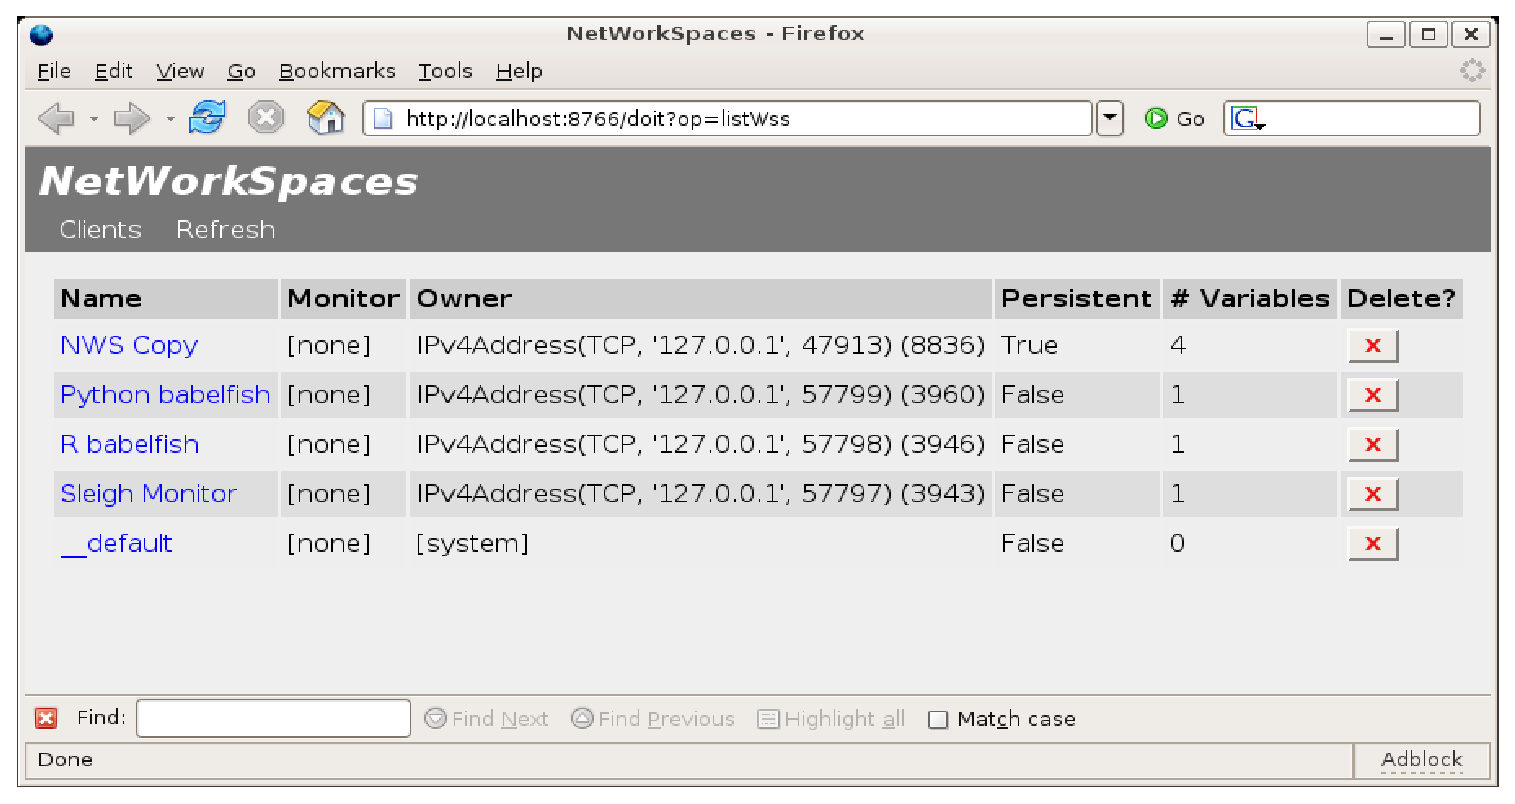
\includegraphics[width=5.95in]{webinterface.eps}

In order to examine the values that you've created from MATLAB in a
workspace using the server's web interface, you'll usually need to have
the MATLAB babelfish running.  The babelfish translates values into a
human readable format so they can be displayed in a web browser.  If a
value is a string, then the web interface simply displays the contents
of the string, without any help from the babelfish, but if the value is
any other type of MATLAB object, it needs help the help of the MATLAB
babelfish.

To run the babelfish, start another MATLAB session on the same machine
that is running the NWS server, and type the following command:

\begin{verbatim}
>> babelfish
\end{verbatim}

Note: this function will not return until you exit your MATLAB session.

For more examples on using NetWorkSpaces, see the Tutorials chapter.

\section{Starting Sleigh}
Sleigh is a MATLAB class, built on top of NetWorkSpaces, that makes it
very easy to write simple parallel programs.  Sleigh has a concept of one
master and multiple workers.  The master sends tasks to the workers who may or
may not be on the same machine as the master.  To enable the master to
communicate with workers, Sleigh supports several mechanisms to launch workers
which execute tasks.

\subsection{Local Launch Mechanism}
The local launch mechanism is the default launch option, and is used for
starting workers on the local machine.  By default, local launch starts
three workers, but you can specify the number of workers to launch by
setting the \texttt{workerCount} variable in the sOpts argument to the
sleigh constructor.  Local launch is useful for developing NetWorkSpace
programs, but it's also the best choice when running on a
multicore/multiprocessor computer.

Here's how to create a Sleigh object:

\begin{samepage}
\begin{verbatim}
>> s = sleigh()
\end{verbatim}
\end{samepage}

This is equivalent to:

\begin{samepage}
\begin{verbatim}
>> sOpts.launch = 'local';
>> s = sleigh(sOpts);
\end{verbatim}
\end{samepage}

\subsection{SSH Launch Mechanism}
To start up workers on machines other than your local computer, you need
to use a remote execution mechanism.  SSH is the most common method on
Unix-like systems.  To use SSH with NetWorkSpaces, set the launch
variable to the \texttt{sshcmd} function, and specify the nodes to run
on with the \texttt{nodeList} option.

For example, here is how you starts workers on the machines 'node1' and
'node2':

\begin{samepage}
\begin{verbatim}
>> sOpts.launch = @sshcmd;
>> sOpts.nodeList = {'node1', 'node2'};
>> s = sleigh(sOpts);
\end{verbatim}
\end{samepage}

You should first configure ssh so that it won't prompt the user for a
password.  This is normally done using the \textit{ssh-agent} program.
See the Appendix B for more information on this.

We don't really recommend using \texttt{sshcmd} on Windows, as
different ssh implementations use various tricks that cause quoting
problems that are very difficult to diagnose.  Nevertheless, we have had
some success using Cygwin's ssh server and copSSH from ITef!x,
\url{http://www.itefix.no/phpws/}.  If you really want to give it a try,
at least avoid using any directories with spaces in them.

\subsection{RSH Launch Mechanism}
RSH can also be used to launch the workers, but it is very insecure, and
SSH should always be preferred.

To start sleigh workers using RSH, the procedure is almost the
same as with SSH:

\begin{samepage}
\begin{verbatim}
>> sOpts.launch = @rshcmd;
>> sOpts.nodeList = {'node1', 'node2'};
>> s = sleigh(sOpts);
\end{verbatim}
\end{samepage}

\subsection{Web Launch Mechanism}
Web launch mechansim allows user to start workers on different
machines in an ad-hoc way, without remote login mechanisms,
such as SSH and RSH. 

To use the web launch option, follow the steps below.

\begin{enumerate}
\item Create an instance of Sleigh:
\begin{samepage}
\begin{verbatim}
>> sOpts.launch = 'web';
>> s = sleigh(sOpts);
\end{verbatim}
\end{samepage}
The Sleigh constructor does not return until it gets a signal that all
workers have started and are ready to accept jobs.
\item Log in to a remote machine.
\item Start a MATLAB session.
\item Open a web browser and point to http://\textit{nwsserver}:8766
\item Click on the newly created Sleigh workspace, and read the value
from variable 'runMe'. It usually has value similar to:\\
\texttt{launch('sleigh\_ride\_004\_tmp', 'n1.xyz.com', 8765);}
\item Copy the 'runMe' value to the MATLAB session. 
\item Repeat steps 2-6 for each worker that needs to be started.
\item Once all workers have started, delete the 'DeleteMeWhenAllWorkers
Started' variable from the Sleigh workspace. This signals
Sleigh master that the workers have started and are ready to accept work. 
\end{enumerate}


\chapter{Tutorials}
\section{Data Sharing Tutorial}
NetWorkSpaces (NWS) is an MATLAB package that makes it very easy to
communicate and coordinate multiple MATLAB programs running on different
machines.  In this chapter, we will give a small walk-through of writing
a simple program using NetWorkSpaces.  Appendix A
contains a detailed reference of the NetWorkSpace class.

First, start an interactive MATLAB session.

Next, create a workspace called `bayport':

\begin{verbatim}
>> ws = netWorkSpace('bayport');
\end{verbatim}

This workspace is created on a NWS server located on localhost, port
8765.  Additional arguments can be passed to the netWorkSpace
constructor to specify a NWS server located on a different host and
port.

\begin{samepage}
\begin{verbatim}
>> opt.host = 'mercury';
>> ws2 = netWorkSpace('bayport', opt);
\end{verbatim}
\end{samepage}

Once we have created a workspace, we can write data into a variable
using the store method:

\begin{verbatim}
>> store(ws, 'joe', 17);
\end{verbatim}

The variable `joe' now has a value of 17 in the workspace named
`bayport'.

To find out the value associates with the variable `joe', we use the
find method:

\begin{verbatim}
>> age = find(ws, 'joe');
\end{verbatim}

which sets `age' to 17.

Note that the find method will block until the variable `joe' has a
value.  This is important when we're trying to read that variable from a
different machine.  If it didn't block, you might have to repeatedly try
to read the variable until it succeeded.  Of course, there are times
when you don't want to block, but just want to see if some variable has
a value.  That is done using the findTry method.

\begin{verbatim}
>> age = findTry(ws, 'chet');
\end{verbatim}

This assigns `0' to age, since we didn't stored any value to variable
`chet'.  If you'd rather have findTry return some other value when the
variable doesn't exist, you can pass in an extra argument to the findTry
method:

\begin{verbatim}
>> age = findTry(ws, 'chet', 1);
\end{verbatim}

which assigns 1 to age, if variable `chet' doesn't exist.

So far, we've carefully executed the store method once for each variable
created.  What if we execute the store method more than once? Then, it
depends on the mode of the variable. By default, a variable created by
the store method uses first-in-first-out (FIFO), which means the first
stored value in the workpace will be the first one to be read. If you
want to use a different mode for the variable, you have to use the
declare method to create the variable first.  Please refer to
Appendix A for a description of the different variable modes.

Since the find method does not remove the value from the workspace, we cannot
use the find method to read multiple values associate with a variable. To
read through all the values, we have to use `fetch' method.  The fetch
method works the same as find, but in addition, it removes the value.
This can be useful in sending a sequence of messages from one program to
another.

Let's try writing multiple values to a variable:

\begin{samepage}
\begin{verbatim}
>> n = [16 19 25 22]
>> for i = 1:length(n)
     store(ws, 'biff', n(i))
   end
\end{verbatim}
\end{samepage}

To read the values, we just call fetch repeatedly:

\begin{samepage}
\begin{verbatim}
>> n = []
>> for i = 1:4
     n = [n fetch(ws, 'biff'))
   end
\end{verbatim}
\end{samepage}

If we didn't know how many values were stored in a variable, we could
have done the following:

\begin{samepage}
\begin{verbatim}
>> n = []
>> while 1
     t = fetchTry(ws, 'biff');
     if t == 0 break; end;
     n = [n t];
   end
\end{verbatim}
\end{samepage}

This uses fetchTry, which works like fetch, except that it is
non-blocking.

These are the basic operations provided by NWS.  It's a good idea to
play around with these operations using two MATLAB sessions.  That way,
you can really transfer data between two different programs.  Also, you
can see how the blocking operations work.  In the examples above, we
were careful never to block because we were only using one MATLAB
session.

To use two MATLAB sessions, just execute MATLAB in another window,
export MATLABPATH or have it saved and load up automatically when a new
window is opened.  Then, open the `bayport' workspace.  This can be done
with the same command that we used previously, but this time, the
command:

\begin{verbatim}
>> ws = netWorkSpace('bayport')
\end{verbatim}

won't create the `bayport' workspace, since it already exists.  Now you
can execute a operation such as:

\begin{verbatim}
>> x = fetch(ws, 'frank')
\end{verbatim}

in one session, watch it block for a minute, and then execute store in
the other session:

\begin{verbatim}
>> store(ws, 'frank', 18)
\end{verbatim}

and see that the fetch in the first session completes.

While you're experimenting with these operations, it can be very helpful
to use the NWS server's web interface to see what's going on in your
workspaces. Just point a web browser to: \url{http://localhost:8766}

If you're using a browser on another machine from the NWS server you'll
have to use the appropriate hostname, rather than `localhost'.

\section{Sleigh for MATLAB Tutorial}
Sleigh is a MATLAB class, built on top of NWS, that makes it very easy to
write simple parallel programs.  It provides two basic functions for
executing tasks in parallel: \textit{eachElem} and \textit{eachWorker}.

\begin{description}
\item[eachElem] is used to execute a specified function multiple times in
parallel with a varying set of arguments.
\item[eachWorker] is used to execute a function exactly once on every worker in
the sleigh with a fixed set of arguments.
\end{description}

\texttt{eachElem} is all that is needed for most basic programs, so that
is what we will start with.

First, we need to start up a sleigh.

\begin{verbatim}
>> s = sleigh
\end{verbatim}

This starts three sleigh workers on the local machine, but the number of
sleigh workers can be changed by specifying workerCount field of the
struct argument. 

Let's shut down sleigh so we can start different number of workers on
local machine. 

\begin{verbatim}
>> stop(s)
\end{verbatim}

This deletes the sleigh's NWS workspace, and shuts down all of the
sleigh worker processes.

Now we'll make a new sleigh, with two workers on local machine, and
we'll use an NWS server that's running on node10:

\begin{samepage}
\begin{verbatim}
>> opt.nwsHost = 'node10';
>> opt.workerCount = 2;
>> s = sleigh(opt)
\end{verbatim}
\end{samepage}

Now we're ready to run a parallel program.  Here it is:

\begin{verbatim}
>> result = eachElem(s, 'add1', 1:10);
\end{verbatim}

In this simple command, we have defined a set of data that is processed
by multiple workers in parallel, and returned each of the results in a
cell array.  Of course, you would never really bother to do such a
trivial amount of work with a parallel program, but you get the idea.

The second argument is the name of the function workers will evaluate.
This assumes that workers have an M function called add1 somewhere in
the system.  If not, you can create a file called `add1.m' with the
content as follows:

\begin{samepage}
\begin{verbatim}
function y = add1(x)
  y = x + 1;
end
\end{verbatim}
\end{samepage}

This eachElem function puts 10 tasks into the sleigh workspace.  Each
task contains one value from 1 to 10.  This value is passed as the
argument to the add1 function.  The return value of the function is put
into the sleigh workspace.  The eachElem function waits for all of the
results to be put into the workspace, and returns them as a cell array,
which are numbers from 2 to 11.

As a second example, let's add two lists together.  We first define an
add2 function, which is written to a file called `add2.m':

\begin{samepage}
\begin{verbatim}
function z = add2(x, y)
  z = x + y;
end
\end{verbatim}
\end{samepage}

Then, we invoke the function with two variable arguments. Since we have two 
variable arguments, we have to wrap them in a cell array:

\begin{verbatim}
>> result = eachElem(s, 'add2', {1:5, 6:10});
\end{verbatim}

This is the parallel equivalent to the MATLAB command:

\begin{verbatim}
>> result = (1:5) + (6:10);
\end{verbatim}

We can keep adding more list arguments in this way, but there is also
a way to add arguments that are the same for every task, which we call
fixed arguments:

\begin{verbatim}
>> result = eachElem(s, 'add2', 1:10, 1);
\end{verbatim}

This is equivalent to the MATLAB command:

\begin{verbatim}
>> result = (1:10) + 1;
\end{verbatim}

It is also equivalent to invoking add1 function we previous defined.
\begin{verbatim}
>> result = eachElem(s, 'add1', 1:10)
\end{verbatim}

The order of the arguments passed to the function are normally in the
specified order, which means that the fixed arguments always come after
the varying arguments.  To change this order, a permutation vector can
be specified.  The permutation vector is specified using the
``argPermute'' field in the execOptions parameter.

For example, to perform the parallel equivalent of the MATLAB operation
100 - (1:10), we do the following:

\begin{samepage}
\begin{verbatim}
>> opt.argPermute = [2 1];
>> result = eachElem(s, 'sub2', 1:10, 100, opt);
\end{verbatim}
\end{samepage}

This permutation vector says to first use the second argument, and then
use the first, thus reverse the order of two arguments.

The sub2.m used in this example looks like this:

\begin{samepage}
\begin{verbatim}
function z = sub2(x, y) 
  z = x - y;
end
\end{verbatim}
\end{samepage}

There is another keyword argument, called ``blocking'', which, if set to
0, will make eachElem return immediately after submitting the tasks,
thus making it non-blocking.  A ``pending'' object is returned, which can
be used periodically to check how many of the tasks are completed, and also
to wait until all tasks are finished.  Here's a quick example:

\begin{samepage}
\begin{verbatim}
>> opt.blocking = 0;
>> sp = eachElem(s, 'add2', {1:1000, 1001:2000}, {}, opt)
>> while check(sp) > 0
     % Do something useful for a little while
   end
>> result = wait(sp)
\end{verbatim}
\end{samepage}

There is also a keyword argument called ``loadFactor'' that enables
watermarking.  This limits the number of tasks that are put into the
workspace at the same time.  This could be important if you're executing
a lot of tasks.  Setting the load factor to 3 limits the number of tasks
in the workspace to 3 times the number of workers in the sleigh workspace.  
Here's how to do it:

\begin{samepage}
\begin{verbatim}
>> opt.loadFactor = 3;
>> result = eachElem(s, 'add2', {1:100, 101:200}, {}, opt);
\end{verbatim}
\end{samepage}

The results are exactly the same as not using a load factor.  Setting
this option only changes the way that tasks are submitted by the
eachElem function.

As you can see, Sleigh makes it very easy to write simple parallel
programs.  But you're not limited to simple programs. You can use NWS
operations to communicate between the worker processes, allowing you to
write message passing parallel programs much more easily than using MPI
or PVM, for example.


\appendix
\chapter{Reference}
\section {netWorkSpace Class}
%HEVEA\aname{netWorkSpace}{
\rule[0.06in]{6in}{0.01in}
\newline
netWorkSpace
\newline
\rule{6in}{0.01in}
\begin{list}{}{}
	\item {\bf Description\\}
	netWorkSpace class constructor.
	\item {\bf Usage\\}
	ws = netWorkSpace(wsName, h, p);
	or \\
	ws = netWorkSpace(wsName, opts);
	\item {\bf Arguments}
 		\begin{tabbing}
		wsName \hspace{2.5cm} \= name of the workspace.\\
		h \> server host name.\\
		p \> server port.\\
		opts \> an optional structure of fields. see details.\\
		\end{tabbing}
	\item {\bf Details\\}
	netWorkSpace(ws, h, p) or netWorkSpace(ws, opts) creates an object for the shared netWorkSpace wsName residing in the netWorkSpaces server 
	running on host h, port p. If host name and port number are not provided, then `localhost' is used as default
	value for host name, and 8765 is used as default value for port.

	opts is an optional structure of fields. If opts is presented, then host name and port number is specified through opts instead
	of arguments to the function.

	opts may contain these fields:
	\begin{itemize}
		\item \textit {server}: nwsServer class object. This field is not needed, if host name and port number are provided. 
		\item \textit {host}: server host name. Default value is `localhost'.
		\item \textit {port}: server port. Default value is 8765. 
		\item \textit {persistent}: If true, make the workspace persistent. A persistent workspace won't be purged when the owner
		disconnects from an nws server. Note that only the client who actually takes ownership of the workspace can make 
		the workspace persistent. The persistent argument is effectively ignored if useUse is true. 
		\item \textit {useUse}: By default `open' semantic is used when creating a workspace (i.e., trying to claim ownership). 
		If useUse is set to 1, `use' semantic applies, which means no ownership is claimed.\\
	\end{itemize}
	
	\item {\bf Examples}
		\begin{verbatim}
		example 1: create a workspace with default options.
		>> nws = netWorkSpace(`nws example')
	
		example 2: connect to a workspace using useUse semantic.
		>> opt.useUse = 1
		>> nws = netWorkSpace(`example2', opt)
	
		example 3: create a workspace on an nws server that
				   resides on node1, port 5555.
		>> nws = netWorkSpace(`example3', `node1', 5555)
		\end{verbatim}
\end{list}
%HEVEA }

%HEVEA\aname{fetch}{
\rule[0.06in]{6in}{0.01in}
\newline
fetch
\newline
\rule{6in}{0.01in}
\begin{list}{}{}
	\item {\bf Description}\\
	Fetch a value associates with the variable from the shared netWorkSpace nws.
	\item {\bf Usage}\\
	X = fetch(nws, varName);
	\item {\bf Arguments}
		\begin{tabbing}
		nws	\hspace{2.5cm} \= a netWorkSpace class object.\\
		varName	\> name of the variable to fetch.\\
		\end{tabbing}
	\item {\bf Details}\\
	Fetch blocks until a value for varName is found in the shared netWorkSpace nws.
	Once found, remove a value associated with varName from the shared netWorkSpace and return it in X. 
	This operation is atomic. If multiple Distributed Computing Toolbox sessions fetch or fetchTry a 
	given varName, any given value from the set of values associated with varName will be return to 
	just one DCT session. If there is more than one value associated with varName, the particular value 
	removed depends on varName's behavior. See declare(nws, ...) for details.
	
	\item {\bf Examples}
		\begin{verbatim}
		>> nws = netWorkSpace(`nws example');
		>> store(nws, `x', 1);  % store variable x with value 1 to nws
		>> X = fetch(nws, `x'); % X = 1
		>> X = fetch(nws, `x'); % no value for x; block on fetch
		\end{verbatim}
\end{list}
%HEVEA}

%HEVEA\aname{fetchTry}{
\rule[0.06in]{6in}{0.01in}
\newline
fetchTry
\newline
\rule{6in}{0.01in}
\begin{list}{}{}
	\item {\bf Description}\\
	Attempt to fetch a value associates with the variable from the shared netWorkSpace nws; 
	a non-blocking version of fetch(nws, ...).
	\item {\bf Usage\\}
	[X, F] = fetchTry(nws, varName, ifMissing);
	\item {\bf Arguments}
		\begin{tabbing}
		nws	\hspace{2.5cm} \= a netWorkSpace class object. \\
		varName	\> name of variable to fetch. \\
		ifMissing \> value to return, if variable by varName is not found in netWorkSpace nws.
		\end{tabbing}
	\item {\bf Details}\\
	Look in the shared netWorkSpace nws for a value bound to varName.
 
	If found, remove a value associated with varName from nws and
	return it in X. Set F to true. This operation is atomic. If
	multiple DCT sessions fetch or fetchTry a given varName, any
	given value from the set of values associated with varName will
	be return to just one DCT session. If there is more than one
	value associated with varName, the particular value removed
	depends on varName's behavior. See declare(nws, ...) for details.
    
	If not found, return the value of ifMissing in X and set F to false.
	Default value for ifMissing is zero. 

	\item {\bf Examples}
		\begin{verbatim}
		>> nws = netWorkSpace(`nws example');
		>> store(nws, `x', 1);
		>> 
		>> [X, F] = fetchTry(nws, `x'); % X = 1, F = 1
		>> [X, F] = fetchTry(nws, `x'); % X = 0, F = 0 
		\end{verbatim}
\end{list}
%HEVEA}

%HEVEA\aname{find}{
\rule[0.06in]{6in}{0.01in}
\newline
find
\newline
\rule{6in}{0.01in}
\begin{list}{}{}
	\item {\bf Description}\\
	Find a value associates with the variable in the shared netWorkSpace nws.
	\item {\bf Usage}\\
	X = find(nws, varName);
	\item {\bf Arguments}
		\begin{tabbing}
		nws	\hspace{2.5cm} \= a netWorkSpace class object. \\
		varName \> name of the variable to find.
		\end{tabbing}
	\item {\bf Details}\\
	find(nws, varName) blocks until a value for varName is found in the shared netWorkSpace nws.
    
	Once found, return in X a value associated with varName, but the value is not removed from
	netWorkSpce, nws. If there is more than one value associated with varName, 
	the particular value returned depends on varName's behavior. See declare(nws, ...) for details.
	\item {\bf Examples}
		\begin{verbatim}
		>> nws = netWorkSpace(`nws example');
		>> store(nws, `x', 1);
		>> X = find(nws, `x');   % X = 1
		>> listVars(nws); % X value is not removed from nws
		\end{verbatim}
\end{list}
%HEVEA }


%HEVEA\aname{findTry}{
\rule[0.06in]{6in}{0.01in}
\newline
findTry
\newline
\rule{6in}{0.01in}
\begin{list}{}{}
	\item {\bf Description}\\
	Attempt to find a value associates with the variable in the shared netWorkSpace nws;	a non-blocking version of find(nws, ...).
	\item {\bf Usage\\}
	[X, F] = findTry(nws, varName, isMissing);
	\item {\bf Arguments}
		\begin{tabbing}
		nws \hspace{2.5cm} \=  a netWorkSpace class object.\\
		varName \> name  of the variable to find.\\
		isMissing \> value to return if no variable by varName is found in netWorkSpace nws.
		\end{tabbing}
	\item {\bf Details}\\
	$[$X, F$]$ = findTry(nws, varName, isMissing) looks in the nws for a value bound to varName.
      
	If found, returns a value associated with varName in X and sets F to true. 
	No value is removed from netWorkSpace, nws. If there is more than one value associated with 
	varName, the particular value returned depends on varName's behavior. 
	See declare(nws, ...) for details.
      
	If not found, return the value of isMissing in X and set F to false.
	Default value for ifMissing is zero. 

	\item {\bf Examples}
		\begin{verbatim}
		>> nws = netWorkSpace(`nws example');
		>> [X, F] = findTry(nws, `x'); % check if variable x exists
		\end{verbatim}
\end{list}
%HEVEA }

%HEVEA\aname{store}{
\rule[0.06in]{6in}{0.01in}
\newline
store
\newline
\rule{6in}{0.01in}
\begin{list}{}{}
	\item {\bf Description}\\
	Store a value associates with the variable in the netWorkSpace, nws.
	\item {\bf Usage}\\
	store(nws, varName, value);
	\item {\bf Arguments}
		\begin{tabbing}
		nws \hspace{2.5cm} \= a netWorkSpace class object.\\
		varName \> variable name.\\
		value \> value associates with varName to be stored in nws. 
		\end{tabbing}
	\item {\bf Details}\\
	store(nws, varName, v) associates the value v with the
	variable varName in the shared netWorkSpace nws, thereby making
	the value available to all the instances of MATLAB running in
	the current Distributed Computing Toolbox session.  value may be
	any MATLAB value -- matrix, structure, function handle, etc.

	If a mode has not already been set for varName, `fifo' will be used (see declare(nws, ...)).

	If no variable name is given, then value v must itself be a variable,
	and the value v will be asssociated with the variable's name in
	the netWorkSpace nws. See the examples below for details.

	Note that, by default (`fifo' mode), store is not idempotent:
	repeating store(nws, `X', v) will add additional values to the
	set of values associated with the name `X'. See the examples below for details.

	\item {\bf Examples}
		\begin{verbatim}
		>> M = magic(5); 
		>> store(nws, M);
		\end{verbatim}
		and
		\begin{verbatim}
		>> store(nws, `M', magic(5));
		\end{verbatim}
		do the same thing. 
	
		\begin{verbatim}
		>> for x = 1:10
		store(nws, `numList', x);
		end
		\end{verbatim}
	
		will associated ten distinct values with the name `numList'.
	
		\begin{verbatim}
		>> for i = 1:10
		fetch(nws, `numList');
		end
		\end{verbatim}
	
		will retrieve these distinct values, one at a time from the
		first to last stored.
\end{list}
%HEVEA }

%HEVEA\aname{declare}{
\rule[0.06in]{6in}{0.01in}
\newline
declare
\newline
\rule{6in}{0.01in}
\begin{list}{}{}
	\item {\bf Description}\\
	Declare a variable with a particular mode in the shared netWorkSpace.
	\item {\bf Usage}\\
	X = declare(nws, varName, mode);
	\item {\bf Arguments}
		\begin{tabbing}
		nws	\hspace{2.5cm} \= a netWorkSpace class object.\\
		varName \> variable name.\\
		mode \>	variable mode.
		\end{tabbing}
	\item {\bf Details}\\
	If varName has not already been declared in nws, the behavior
	of varName will be determined by mode. Mode can be `fifo',
	`lifo', `multi', or `single'. In the first three cases,
	multiple values can be associated with varName. When a value is
	retrieved for varName, the oldest value stored will be used in
	`fifo' mode, the youngest in `lifo' mode, and a
	nondeterministic choice will be made in `multi' mode. In
	`single' mode, only the most recent value is retained.
	\item {\bf Examples}
		\begin{verbatim}
		>> nws = netWorkSpace(`nws example');
		>> declare(nws, `pi', `single');
		>> store(nws, `pi', 2.171828182);
		>> store(nws, `pi', 3.141592654);
		\end{verbatim}

	listVars(nws) will show that only the most recent value of pi is retained.
\end{list}
%HEVEA }

%HEVEA\aname{deleteVar}{
\rule[0.06in]{6in}{0.01in}
\newline
deleteVar
\newline
\rule{6in}{0.01in}
\begin{list}{}{}
	\item {\bf Description}\\
	Delete a variable from the shared netWorkSpace.
	\item {\bf Usage}\\
	X = deleteVar(nws, varName);
	\item {\bf Arguments}
		\begin{tabbing}
		nws \hspace{2.5cm} \= a netWorkSpace class object.\\
		varName \> variable name of the object to delete.
		\end{tabbing}
	\item {\bf Examples}
		\begin{verbatim}
		>> nws = netWorkSpace(`nws example');
		>> store(nws, `x', 1);
		>> deleteVar(nws, `x');
		>> listVars(nws); % no variables in nws example 
		\end{verbatim}
\end{list}
%HEVEA }

%HEVEA\aname{listVars}{
\rule[0.06in]{6in}{0.01in}
\newline
listVars
\newline
\rule{6in}{0.01in}
\begin{list}{}{}
	\item {\bf Description}\\
	List variables in the netWorkSpace, nws.
	\item {\bf Usage}\\
	X = listVars(nws, netWorkSpaceName);
	\item {\bf Arguments}
		\begin{tabbing}
		nws \hspace{3.0cm} \= a netWorkSpace class object.\\
		netWorkSpaceName \> netWorkSpace name.
		\end{tabbing}
	\item {\bf Details}\\
	X = listVars(netWorkSpaceName) returns a struct array listing
	of variables in the named netWorkSpace. The listing contains number of values,
	fetchers, finders and mode for each variable. If netWorkSpaceName argument
        is not provided, then list variables in the netWorkSpace reference by the first argument, nws. 
     
	If no left hand side, print a tabular listing.
	\item {\bf Examples}
		\begin{verbatim}
		>> nws = netWorkSpace(`nws example');
		>> store(nws, `x', 1);
		>> listVars(nws);
		\end{verbatim}
\end{list}
%HEVEA }

%HEVEA\aname{currentWs}{
\rule[0.06in]{6in}{0.01in}
\newline
currentWs
\newline
\rule{6in}{0.01in}
\begin{list}{}{}
	\item {\bf Description}\\
	Report the name of a shared netWorkSpace.
	\item {\bf Usage}\\
	X = currentWs(nws);
	\item {\bf Arguments}
		\begin{tabbing}
		nws	\hspace{2.5cm} \= a netWorkSpace class object.
		\end{tabbing}
	\item {\bf Examples}
		\begin{verbatim}
		>> nws = netWorkSpace(`nws example');
		>> wsName = currentWs(nws);
		>> display(wsName); % wsName = nws example 
		\end{verbatim}
\end{list}
%HEVEA }

%HEVEA\aname{close}{
\rule[0.06in]{6in}{0.01in}
\newline
close
\newline
\rule{6in}{0.01in}
\begin{list}{}{}
	\item {\bf Description}\\
	Close connection of a shared netWorkSpace to the NetWorkSpaces server. 
	\item {\bf Usage}\\
	X = close(nws);
	\item {\bf Arguments}
		\begin{tabbing}
		nws \hspace{2.5cm} \= a netWorkSpace class object.
		\end{tabbing}
	\item {\bf Examples}
		\begin{verbatim}
		>> nws = netWorkSpace(`nws example');
		>> close(nws);
		\end{verbatim}
\end{list}
%HEVEA }

%HEVEA\aname{server}{
\rule[0.06in]{6in}{0.01in}
\newline
server
\newline
\rule{6in}{0.01in}
\begin{list}{}{}
	\item {\bf Description}\\
	Return an instance of the NetWorkSpaces server that the netWorkSpace, nws, connects to.
	\item {\bf Usage}\\
	s = server(nws);
	\item {\bf Arguments}
		\begin{tabbing}
		nws \hspace{2.5cm} \= a netWorkSpace class object.
		\end{tabbing}
	\item {\bf Examples}
		\begin{verbatim}
		>> s = server(nws);
		\end{verbatim}
\end{list}
%HEVEA }


\section {nwsServer Class}
%HEVEA\aname{nwsServer}{
\rule[0.1in]{6in}{0.01in}
\newline
nwsServer
\newline
\rule{6in}{0.01in}
\begin{list}{}{}
	\item {\bf Description}\\
	nwsServer class constructor.
	\item {\bf Usage}\\
	nwss = nwsServer(h, p)
	\item {\bf Arguments}
		\begin{tabbing}
		h \hspace{2.5cm} \= server host name. Default is `localhost'.\\
		p \> server port number. Default is 8765.
		\end{tabbing}
	\item {\bf Examples}
	\begin{verbatim}
	example 1: create a nws server with default options.
	>> nwss = nwsServer;   % create nws server with default options
	
	example 2: create a nws server on node1, port 5000.
	>> nwss = nwsServer(`node1', 5000);
	\end{verbatim}
\end{list}
%HEVEA }

%HEVEA\aname{openWs}{
\rule[0.06in]{6in}{0.01in}
\newline
openWs
\newline
\rule{6in}{0.01in}
\begin{list}{}{}
	\item {\bf Description}\\
	Create a netWorkSpace class object. 
	\item {\bf Usage}\\
	nws = openWs(nwss, netWorkSpaceName, opts);
	\item {\bf Arguments}
		\begin{tabbing}
		nwss \hspace{2.5cm} \= a nwsServer class object. \\
		netWorkSpaceName \> name of the netWorkSpace to open.\\
		opts \> a structure of optional fields.
		\end{tabbing}
	\item {\bf Details}\\
	openWs(nwss, netWorkSpaceName) creates a shared netWorkSpace object for
	the netWorkSpace named netWorkSpaceName (which must be a string). 
	If the shared netWorkSpace does not exist, it will be created (upon first use)
	and claimed the ownership of the workspace. This can be useful as an arbitration
	mechanism. The output of listWss indicates which netWorkSpace this MATLAB process
	created. These will be destroyed when this MATLAB process closes the connection
	to the netWorkSpace server that was used to create these spaces, except when 
        when they are persistent workspaces. \\

	opts argument has two optional fields: 
	\begin{itemize}
	\item \textit {persistent}: a boolean value indicating whether the workspace is persistent or not. If
	the workspace is persistent (value of 1), then the workspace is not purged
	when the owner disconnects from the server. Default value is 0.
	\item \textit {space}: a netWorkSpace class object. 
	If this field is specified, then the existing netWorkSpace and server connection are used. Otherwise, a new netWorkSpace 
    class object with the connection to the nws server, nwss, is created.
	\end{itemize}
	
	\item {\bf Examples}
	\begin{verbatim}
	example 1: open a workspace with default options.
	>> nwss = nwsServer;
	>> nws = openWs(nwss, `my space');
	
	example 2: open a persistent workspace.
	>> nws2 = openWs(nwss, `my space2', opt);
	\end{verbatim}
\end{list}
%HEVEA }

%HEVEA\aname{useWs}{
\rule[0.06in]{6in}{0.01in}
\newline
useWs
\newline
\rule{6in}{0.01in}
\begin{list}{}{}
	\item {\bf Description}\\
	Connect to a shared netWorkSpace, but not own it. 
	\item {\bf Usage}\\
	nws = useWs(nwss, netWorkSpaceName, opts);
	\item {\bf Arguments}
		\begin{tabbing}
		nwss \hspace{3.0cm} \= a nwsServer class object. \\
		netWorkSpaceName \> name of the netWorkSpace to open.\\
		opts \> a structure of optional fields.
		\end{tabbing}
	\item {\bf Details}\\
	useWs(nwss, netWorkSpaceName, opts) creates a shared netWorkSpace object
	for the netWorkSpace named netWorkSpaceName (which must be a string).
	If the shared netWorkSpace does not exist, it will be created but no owner
	associates with it. \\
	
	opts argument contains the following field:
	\begin{itemize}
	\item \textit{space}: a netWorkSpace object that represents the workspace that client wants to `use', but not own. 
	If this field is specified, then the existing netWorkSpace and server connection are used. Otherwise, a new netWorkSpace 
    class object with the connection to the nws server, nwss, is created.
	\end{itemize}
		
	\item {\bf Examples}
	\begin{verbatim}
	>> nwss = nwsServer;
	>> nws = useWs(nwss, `my space');
	\end{verbatim}
\end{list}
%HEVEA }

%HEVEA\aname{listWss}{
\rule[0.06in]{6in}{0.01in}
\newline
listWss
\newline
\rule{6in}{0.01in}
\begin{list}{}{}
	\item {\bf Description}\\
	List all netWorkSpaces in the nwsServer, nwss.
	\item {\bf Usage}\\
	X = listWss(nwss);
	\item {\bf Arguments}
		\begin{tabbing}
		nwss \hspace{2.5cm} \= a nwsServer class object.
		\end{tabbing}
	\item {\bf Details}\\
	X = listWss(nwss) returns a struct array listing information
	about all the netWorkSpaces currently available on the server reached by connection nwss.

	If no left hand side, print a tabular listing. 
		
	\item {\bf Examples}
	\begin{verbatim}
	>> nws = netWorkSpace(`my space');
	>> store(nws, `a', 1);
	>> store(nws, `b', 2);
	>> nwss = server(nws);
	>> listWss(nwss);
	\end{verbatim}
\end{list}
%HEVEA }

%HEVEA\aname{mktempWs}{
\rule[0.06in]{6in}{0.01in}
\newline
mktempWs
\newline
\rule{6in}{0.01in}
\begin{list}{}{}
	\item {\bf Description}\\
	Create a unique temporary workspace using template string.

	\item {\bf Usage}\\
	name = mktempWs(nwss, wsNameTemplate);

	\item {\bf Arguments}
		\begin{tabbing}
		nwss \hspace{2.5cm} \= a nwsServer class object. \\
		wsNameTemplate \> template for the netWorkSpace name.
		\end{tabbing}
	\item {\bf Details}\\
	name = mktempWs(nwss, wsNameTemplate) returns the name of a temporary space created
	on the server reached by nwss. The template should contain a `\%d'-like construct
	which will be replaced by a serial counter maintained by the server to generate
	a unique new workspace name. The user must then invoke openWs() or useWs() with this name
	to create a netWorkSpace object to access this workspace. wsNameTemplate defaults to `matlab\_ws\_\%010d'.
		
	\item {\bf Examples}
	\begin{verbatim}
	>> nwss = nwsServer;
	>> nws = mktempWs(nwss, `template_%010d');
	\end{verbatim}
\end{list}
%HEVEA }

%HEVEA\aname{socket}{
\rule[0.06in]{6in}{0.01in}
\newline
socket
\newline
\rule{6in}{0.01in}
\begin{list}{}{}
	\item {\bf Description}\\
	returns socket connection of a nwsServer, nwss.	
	\item {\bf Usage}\\
	s = socket(nwss);
	\item {\bf Arguments}
		\begin{tabbing}
		nwss \hspace{2.5cm} \= a nwsServer class object.
		\end{tabbing}	
	\item {\bf Examples}
	\begin{verbatim}
	>> nwss = nwsServer;
	>> socket(nwss);
	\end{verbatim}
\end{list}
%HEVEA }

%HEVEA\aname{deleteWs}{
\rule[0.06in]{6in}{0.01in}
\newline
deleteWs
\newline
\rule{6in}{0.01in}
\begin{list}{}{}
	\item {\bf Description}\\
	Delete a shared netWorkSpace with specific name from the nwsServer, nwss. 
	\item {\bf Usage}\\
	X = deleteWs(nwss, wsName);
	\item {\bf Arguments}
		\begin{tabbing}
		nwss \hspace{2.5cm} \= a nwsServer class object. \\
		wsName \> name of netWorkSpace.
		\end{tabbing}	
	\item {\bf Examples}
	\begin{verbatim}
	>> nwss = nwsServer;
	>> deleteWs(nwss, `my space');
	\end{verbatim}
\end{list}
%HEVEA }

\section {Sleigh Class}
%HEVEA\aname{sleigh}{
\rule[0.06in]{6in}{0.01in}
\newline
sleigh
\newline
\rule{6in}{0.01in}

\begin{list}{}{}
	\item {\bf Description}\\
	  Sleigh class constructor.  
	\item {\bf Usage}\\
	  s = sleigh(sOpts);
	\item {\bf Arguments}
		\begin{tabbing}
		sOpts \hspace{2.0cm} \= an optional structure of fields, see Details.\\
		\end{tabbing}
	\item {\bf Details}\\
     s = sleigh brings up three workers on `localhost' with default options for sOpts argument.
     
     sOpts argument contains several fields that give you ability to customize sleigh objects. 
     
	 \begin{itemize}
	        \item \textit {nodeList}: a cell array of hosts on which to execute workers. One worker
		  is created for each of the host names in the cell array. The default value is {`localhost', `localhost', `localhost'},
		  which starts up three workers on local machine. nodeList is ignored when local launch or web launch is used. 
		\item \textit {workerCount}: an integer that indicates how many workers will be created. Default value is 3.
		  This variable is only relevant for local launch. 
		\item \textit {nwsHost}: netWorkSpace server host name. Default is local machine. 
		\item \textit {nwsPort}: netWorkSpace server port. Default port is 8765.
		\item \textit {nwsPath}: directory path of where nws package is installed on worker nodes. Default is set to where NWS MATLAB is installed on the master node. This field is irrelevant to web launch.
		\item \textit {outfile}: all remote workers' output will be redirected to this file, if verbose mode is set. By default, this field does not exist.
		\item \textit {launch}: mechanism to launch workers. Four mechanisms are supported: ssh, rsh, web and local. For local and web, set launch to a string
		  `local' and `web' respectively. For ssh and rsh, set launch to an anonymous function @sshcmd and @rshcmd respectively. 
		\item \textit {scriptDir}: directory where matlab worker script is stored. Default is set to the bin directory under NWS MATLAB directory. This field is irrelevant to web launch.
		\item \textit {scriptName}: script file name. Default is MatlabNWSSleighSession.sh on UNIX and MatlabNWSSleighSession.py for Windows.
		\item \textit {user}: user name for remote login. This argument may be ignored depending on the launch type. 
		  Default is the value set by environment variable, USER, on the sleigh master.
		\item \textit {workingDir}: define remote workers' working directory. By default, this field is seet to master sleigh's current directory. 		\item \textit {logDir}: define the directory where log files are stored. By default, this field does not exist. 
		\item \textit {wsNameTemplate}: template for the sleigh workspace name. This must be a legal `format' string, containing only an integer format specifier. Default prefix is `sleigh\_ride\_\%010d'
		\item \textit {verbose}: verbose mode (0 or 1). Default value is 0. 
    \end{itemize}
         	    
	\item {\bf Examples}
		\begin{verbatim}
		example 1:  start sleigh workers with default options.
		>> s = sleigh;		

		example 2:  create two sleigh workers on local machine using local launch, 
                            and have server running on node10.
		>> opt.nwsHost = `node10';
		>> opt.workerCount = 2;
		>> s = sleigh(opt);
     
		example 3: create two workers on node1 and node2 using ssh.
		>> opt.launch = @sshcmd;
		>> opt.nodeList = {`node1', `node2'};
		>> s = sleigh(opt);

		example 4: start sleigh with web launch.
		>> opt.launch = `web';
		>> s = sleigh(opt);
		\end{verbatim}
\end{list}
%HEVEA }

%HEVEA\aname{eachWorker}{
\rule[0.06in]{6in}{0.01in}
\newline
eachWorker
\newline
\rule{6in}{0.01in}
\begin{list}{}{}
	\item {\bf Description}\\
     Evaluates function exactly once for each worker in sleigh, s. 
	\item {\bf Usage}\\     
     x = eachWorker(s, toDo, fixedArgs, execOptions);
	\item {\bf Arguments}
		\begin{tabbing}
		s \hspace{2.0cm} \= a sleigh class object.\\
		toDo \> function or expression to be evaluated by sleigh workers. \\
		varargin \> fixed arguments or/and a structure of options.
		\end{tabbing}
		
	\item {\bf Details}\\  
    The only required arguments for eachWorker are s and toDo. The rest are optional arguments. 
    
    varargin is a variable length of arguments. It is used to specify fixed arguments followed by a structure of fields. 
    For sleigh workers, arguments passed to the evaluated function or expression can be accessed through a global variable named sleighTask.argCA, 
    which is a cell array of values mapped from varargin. The last element of varargin can be a structure that contains the following fields:
  	\begin{itemize}
		\item \textit{type}: determines the type of function invocation. This can be `invoke' (evaluate the function), 
		`define' (transport function to sleigh workers, no evaluation will be done), or `eval' (evaluate expression).
		Default type is `invoke'. If type is `invoke' or `define', then toDo argument must be a valid function name. 
		If type is `eval', then toDo argument is evaluated as it is. 
		\item \textit{blocking}: determines whether to wait for the results, or to return as soon as the tasks have submitted. 
		Default value is set to 1, which means eachWorker is blocked until all tasks are completed. If value
		is set to 0, then eachWorker returns immediately with a sleighPending object that is used to monitor the 
		status of the tasks, and eventually used to retrieve results. You must wait for the results to be completed
		before submitted more tasks to the sleigh workspace. 
	\end{itemize}

    The results from eachWorker are returned as a two-dimensional cell array.
    However, if blocking field of the structure is set to 0, then an instance of the sleighPending class is returned.
    
	\item {\bf Examples}
		\begin{verbatim}
		example 1: execute function with no arguments.
		>> s = sleigh;
		>> status = eachWorker(s,`init');

		Here is how init.m may look like: 
		function x = init()
		x = 1;
                end

		example 2: execute eachWorker with eval execution type.
		>> s = sleigh;
		>> opt.type=`eval'
		>> eachWorker(s, `2*sleighTask.argCA{1}', 3, opt)	
		\end{verbatim}
\end{list}
%HEVEA }

%HEVEA\aname{eachElem}{
\rule[0.06in]{6in}{0.01in}
\newline
eachElem
\newline
\rule{6in}{0.01in}
\begin{list}{}{}
	\item {\bf Description}\\
	Evaluate multiple argument sets using workers in sleigh, s. 
	\item {\bf Usage\\}
	x = eachElem(s, toDo, elementArgs, fixedArgs, execOptions);
	\item {\bf Arguments}
		\begin{tabbing}
		s \hspace{2.5cm} \= a sleigh class object.\\
		toDo \> function or expression to be evaluated by sleigh workers. \\
		elementArgs \> a vector, a cell array of elements (x, y, ... z), or two dimensional cell arrays. \\
		fixedArgs \> a scalar or a cell array of fixed arguments/constants \\
		execOptions \> an optional structure of fields.
		\end{tabbing}

	\item {\bf Details}\\
	  eachElem(s, toDo, elementArgs, fixedArgs, execOptions) forms argument sets from values passed in elementArgs and fixedArgs. 
	  elementArgs can be a vector, a cell array of entries (x, y, ... z), or a two-dimensional cell array. 
	  If elementArgs is a single-dimensional cell array with entries (x, y, ... z), 
	  then all entries must be of same length, which is determined by the iterating scheme (variable 'by' in execOptions struct). 
	  For example, if iterating schemes is to iterate by row, then then the number of rows for each argument has to be equal. 

	  If function to be executed requires only one varying argument, then elementArgs can be
	  expressed as a vector instead of a cell array. 

	  If elementArgs is a two-dimensional cell array, then the number of tasks equals
	  the number of rows in a two-dimensional cell array. The number of arguments to the 
	  function equals the number of columns in the two-dimensional cell array.
 
	  If fixedArgs is provided, then these additional arguments are appended to the argument set. 
	  The ordering of arguments can be changed by using argPermute vector, which defined as part of 
	  execOptions (see below).

	  The results from eachElem are normally returned as a two-dimensional cell array. 
	  However, if blocking field of execOptions is set to 0, then an instance of the sleighPending class is returned.

	  toDo argument is a function or an expression to be evaluated by sleigh workers. toDo must be a function name (for `invoke'
	  type) or expressions (for `eval' type) in quotes.
    
	  For sleigh workers, arguments passed to the evaluated function or expression can be accessed through a global variable named sleighTask.argCA, 
          which is a cell array of values concatenate together from elementArgs and fixedArgs.

	  execOptions argument is a structure that contains the following fields:
	\begin{itemize}
		\item \textit {type}: determines the type of function invocation to perform. This can be `invoke' (evaluate the function) or 
		`eval' (evaluate expression). Default type is `invoke'. If type is `invoke', then toDo argument must be a valid function name.
		If type is `eval', then toDo argument is evaluated as is. 
    
		\item \textit {blocking}: determines whether to wait for the results, or to return as soon as the tasks have submitted. 
		Default value is set to 1, which means eachElem is blocked until all tasks are completed. If value is set to 0,
		then eachElem returns immediately with a sleighPending object that is used to monitor the status of the tasks,
		and eventually used it to retrieve results. You must wait for the results to be completed before submitting
		more tasks to the sleigh workspace.
	
		\item \textit {argPermute}: a vector of integers used to permute each (elementArgs + fixedArgs) argument list to match 
		the calling convention of toDo.
    
		\item \textit {loadFactor}: to restrict the number of tasks put out to the workspace.
		If set, no more than loadFactor times the number of worker tasks will be posted at once.
                This helps to control resource demands on the nws server. It is mutually exclusive with
                `blocking' set to 0.

		\item \textit {by}:  one of three iterating schemes: `cell', `row', or
		  `column'. Default value is to iterate by cell. All elements of
		  elementArgs iterates based on the 'by' value. If different
		  iterating scheme is needed for each element of the
		  elementArgs, a cell array of different iterating schemes can
		  be specified. For example: opt.by = {'row', 'column'}.
		  Each index of the 'by' cell array represents the iterating
		  scheme for the corresponding elements in the elementArgs. 
		  If no value is specified, then default value `cell' is assumed. 
		  The `by' field is ignored if elementArgs is a two-dimensional cell array.

	\end{itemize}
    
	\item {\bf Examples}\\
	Here is how addone.m may look like:
		\begin{verbatim}
		>> s = sleigh;
		>> result = eachElem(s, `mean', {[1 2.5 3.1]})

		result =
		    [     1]
  		    [2.5000]
		    [3.1000]
		\end{verbatim}	

		eachElem(s, `foo', {1:3, 4:6, 7:9})\\

		will generate three invocations of `foo':\\

			foo(1, 4, 7)\\
			foo(2, 5, 8)\\
			foo(3, 6, 9)\\

		while

		\begin{verbatim}
		elementArgs = {1:3, 4:6, 7:9}
		fixedArgs = {100, 200, 300}
		eachElem(s, `foo', elementArgs, fixedArgs)
		\end{verbatim}

		will generate:\\

		foo(1, 4, 7, 100, 200, 300)\\
		foo(2, 5, 8, 100, 200, 300)\\
		foo(3, 6, 9, 100, 200, 300)\\
        
        To change invocation type
	
		\begin{verbatim}
		>> opt.type = `eval'
		>> eachElem(s, `sleighTask.argCA{1}*2', 1:5, {}, opt);
		ans = 
		    [2]
		    [4]
		    [6]
		    [8]
		    [10]
		\end{verbatim}
		
		To change the order of passing arguments
	
		\begin{verbatim}
		>> opt.argPermute = [1 3 2 6 5 4]
		>> opt.type = `invoke'
		>> eachElem(s, `foo', elementArgs, fixedArgs)
		\end{verbatim}
	    
		will generate:\\
	 
			foo(1, 7, 4, 300, 200, 100)\\
			foo(2, 8, 5, 300, 200, 100)\\
			foo(3, 9, 6, 300, 200, 100)\\
\end{list}
%HEVEA }

%HEVEA\aname{nws}{
\rule[0.06in]{6in}{0.01in}
\newline
nws
\newline
\rule{6in}{0.01in}
\begin{list}{}{}
	\item {\bf Description}\\
	Return the netWorkSpace that is used to communicate data between sleigh master and sleigh workers. 
	\item {\bf Usage}\\
	nws(s);
	\item {\bf Arguments}
		\begin{tabbing}
		s \hspace{2.5cm} \= a sleigh class object.
		\end{tabbing}
	\item {\bf Examples}
		\begin{verbatim}
		>> s = sleigh
		>> nws(s)
		\end{verbatim}
\end{list}
%HEVEA }

%HEVEA\aname{stop}{
\rule[0.06in]{6in}{0.01in}
\par
stop
\newline
\rule{6in}{0.01in}
\begin{list}{}{}
	\item {\bf Description}\\
	Remove worker processes and delete the sleigh workspace.
	\item {\bf Usage}\\
	stop(s)
	\item {\bf Arguments}
		\begin{tabbing}
		s \hspace{2.5cm} \= a sleigh class object.\\
		\end{tabbing}
	\item {\bf Examples}
		\begin{verbatim}
		>> s = sleigh
		>> stop(s)
		\end{verbatim}
\end{list}
%HEVEA }


\section {sleighPending Class}
%HEVEA\aname{sleigh}{
\rule[0.06in]{6in}{0.01in}
\newline
sleighPending
\newline
\rule{6in}{0.01in}
\begin{list}{}{}
	\item {\bf Description}\\
	  sleighPending class constructor.  
	\item {\bf Usage}\\
	  s = sleigh(nws, count, tb, busyfh);
	\item {\bf Arguments}
		\begin{tabbing}
		nws \hspace{2.0cm} \= netWorkSpace class object.\\
		count \> number of tasks.\\
		tb \> barrier names.\\
		busyfh \> sleigh state.\\	
		\end{tabbing}
	\item {\bf Details}\\
     sp = sleighPending(nws, count, tb, busyfh) creates a pending sleigh job, sp. 
     The sleighPending object can be used to monitor outstanding tasks and to 
     retrieve results upon completion. 
         	    
	\item {\bf Examples}
		\begin{verbatim}
		example 1:  
		get sleighPending object from non-blocking eachElem
		>> opts.blocking = 0;
		>> s = sleigh;
		>> sp = eachElem(s, 'add1', 1:1000, {}, opts)
		\end{verbatim}
\end{list}
%HEVEA }


%HEVEA\aname{check}{
\rule[0.06in]{6in}{0.01in}
\newline
check
\newline
\rule{6in}{0.01in}
\begin{list}{}{}
	\item {\bf Description}\\
    Return the number of results yet to be generated for the pending sleigh job, sp. 
	\item {\bf Usage}\\
	check(sp);
	\item {\bf Arguments}
		\begin{tabbing}
		sp \hspace{2.5cm} \= a sleighPending class object.
		\end{tabbing}
	\item {\bf Details}\\
	The pending sleigh job, sp, is usually obtained through non-blocking eachElem or non-blocking eachWorker. 
	If the job has already completed and the results have been gathered, 0 is returned. 
	\item {\bf Examples}
		\begin{verbatim}
		>> s = sleigh
		>> opt.blocking = 0
		>> sp = eachElem(s, `addone', 1:1000, {}, opt)
		>> check(sp)
		\end{verbatim}
\end{list}
%HEVEA }

%HEVEA\aname{wait}{
\rule[0.06in]{6in}{0.01in}
\newline
wait
\newline
\rule{6in}{0.01in}
\begin{list}{}{}
	\item {\bf Description}\\
    Wait and block for the results to be completed for the pending sleigh job, sp. 
    If the job has already completed, then wait returns immediately with generated results. 
	\item {\bf Usage}\\
	wait(sp);
	\item {\bf Arguments}
		\begin{tabbing}
		sp \hspace{2.5cm} \= a sleighPending class object.
		\end{tabbing}
	\item {\bf Details}\\
	The pending sleigh job, sp, is usually obtained from the return value of non-blocking eachElem or non-blocking eachWorker. 
	\item {\bf Examples}
		\begin{verbatim}
		>> s = sleigh
		>> opt.blocking = 0
		>> sp = eachElem(s, `addone', 1:1000, {}, opt)
		>> wait(sp)
		\end{verbatim}
\end{list}
%HEVEA }


\chapter{Remote Execution Configuration}
\section{Setting Up a Password-less SSH Login}
\begin{itemize}
\item To generate public and private keys, follow the steps below:
\begin{itemize}
\item Open a terminal (shell on UNIX and DOS prompt on Windows).
\item \texttt{ssh-keygen -t rsa} \\ (assume ssh-keygen is in your PATH)
\item \texttt{cd .ssh} \\ (.ssh directory is located in your HOME directory,
/home/user on UNIX or Cygwin and
C:$\backslash$Program~Files$\backslash$copssh$\backslash$home$\backslash$user on Windows)
\item \texttt{cp id\_rsa.pub authorized\_keys} \\
This step allows password-less login to local machine. 
\item For all remote machines that you want password-less login, append the content of 
id\_rsa.pub to their authorized\_keys file.
\end{itemize}
\item To test the password-less login, type the following command:
\begin{verbatim}
% ssh hostname date
\end{verbatim}
If everything is setup correctly, you should not be asked for password and the
current date on remote machine will be returned. 
\end{itemize}


\end{document}
